\documentclass[12pt]{article}
\usepackage[english]{babel}
\usepackage[utf8]{inputenc}
\usepackage{amsmath, amssymb, amsthm}
\usepackage{graphicx}
\usepackage{hyperref}
\usepackage{geometry}
\usepackage{xcolor}
\usepackage{tikz}

\setlength{\topmargin}{0pt}
\setlength{\headsep}{0pt}
\textheight = 600pt

\title{Graph Theory \\ Homework 1}
\author{Ben Kallus and Maddy LaPoint}
\date{Due Friday, February 5}

\begin{document}
\pagecolor{black}
\color{white}
\maketitle

\noindent{\bf 1.1}

    After reading Example 1.1, the next logical question to ask is whether it is possible to have all seven committees meet without conflict in the three time slots.
    This is possible since, for example, $c_1$, and $c_4$ can meet in the first time slot, $c_7$ and $c_3$ can meet in the second time slot, and $c_6$, $c_2$, and $c_5$ can meet in the third time slot.


\bigskip
\noindent{\bf 1.4}

    $G:$

    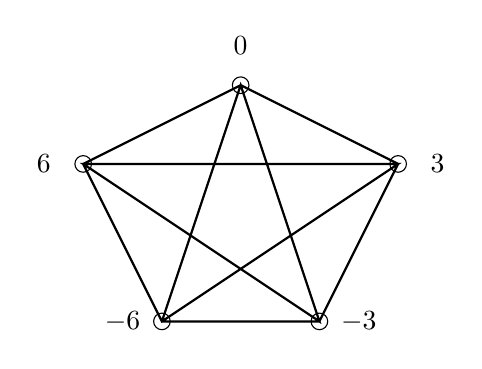
\begin{tikzpicture}
        %% vertices
        \draw[fill=white] (1,0) circle (3pt);
        \draw[fill=white] (3,0) circle (3pt);
        \draw[fill=white] (4,2) circle (3pt);
        \draw[fill=white] (2,3) circle (3pt);
        \draw[fill=white] (0,2) circle (3pt);
        %% vertex labels
        \node at (0.5,0) {$-6$};
        \node at (3.5,0) {$-3$};
        \node at (4.5,2) {$3$};
        \node at (2,3.5) {$0$};
        \node at (-0.5,2) {$6$};
        %% edges
        \draw[thick] (1,0) -- (3,0) -- (4,2) -- (2,3) -- (0,2) -- (1,0) -- (4,2) -- (0,2) -- (3,0) -- (2,3) -- (1,0);
    \end{tikzpicture}

\newpage
\noindent{\bf 1.6}
    
    $F:$
    \bigskip

    \newcommand{\cone}{(-.5,-.5)}
    \newcommand{\ctwo}{(1,-4)}
    \newcommand{\cthree}{(-1,-4)}
    \newcommand{\cfour}{(.5,-.5)}
    \newcommand{\cfive}{(-3,-2)}
    \newcommand{\csix}{(-3,0)}
    \newcommand{\cseven}{(.5,-1.5)}
    \newcommand{\ceight}{(-1,2)}
    \newcommand{\cnine}{(1,2)}
    \newcommand{\cten}{(-.5,-1.5)}
    \newcommand{\celeven}{(3,0)}
    \newcommand{\ctwelve}{(3,-2)}

    \begin{tikzpicture}
        %% vertices
        \draw[fill=white] \cone circle (3pt);
        \draw[fill=white] \ctwo circle (3pt);
        \draw[fill=white] \cthree circle (3pt);
        \draw[fill=white] \cfour circle (3pt);
        \draw[fill=white] \cfive circle (3pt);
        \draw[fill=white] \csix circle (3pt);
        \draw[fill=white] \cseven circle (3pt);
        \draw[fill=white] \ceight circle (3pt);
        \draw[fill=white] \cnine circle (3pt);
        \draw[fill=white] \cten circle (3pt);
        \draw[fill=white] \celeven circle (3pt);
        \draw[fill=white] \ctwelve circle (3pt);
        %% vertex labels
        \node at (-.25,-.5-.25) {$c_1$};
        \node at (1,-4-.5) {$c_2$};
        \node at (-1,-4-.5) {$c_3$};
        \node at (.25,-.5-.25) {$c_4$};
        \node at (-3,-2+.5) {$c_5$};
        \node at (-3,0+.5) {$c_6$};
        \node at (.25,-1.5+.25) {$c_7$};
        \node at (-1,2+.5) {$c_8$};
        \node at (1,2+.5) {$c_9$};
        \node at (-.25,-1.5+.25) {$c_{10}$};
        \node at (3,0+.5) {$c_{11}$};
        \node at (3,-2+.5) {$c_{12}$};
        %% edges
        \draw[thick] \cone -- \cfive -- \cten -- \ctwo -- \cseven -- \cthree -- \cten -- \csix -- \cone -- \ceight -- \cfour -- \cnine -- \cone;
        \draw[thick] \cfour -- \celeven -- \cseven -- \ctwelve -- \cfour;
    \end{tikzpicture}

\bigskip
\noindent{\bf 1.8(a)}
    
    \begin{align*}
        S_1 &= \{\text{fob}, \text{cob}, \text{cot}, \text{tot}\} \\
        S_2 &= \{\text{pup}, \text{ump}, \text{pump}, \text{pomp}\} \\
        S_3 &= \{\text{tap}, \text{sap}, \text{lap}, \text{clap}\} \\
        S_4 &= \{\text{rope}, \text{dope}, \text{rote}, \text{dote}\} \\
        S_5 &= \{\text{slip}, \text{lip}, \text{sip}, \text{tip}\} \\
        S_6 &= \{\text{pop}, \text{top}, \text{lop}, \text{sop}\}
    \end{align*}

\newpage
\noindent{\bf 1.11}

    $G - X:$

    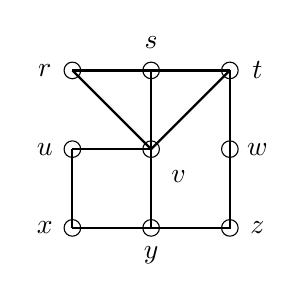
\begin{tikzpicture}
        \draw[fill=white] (0,0) circle (3pt);
        \draw[fill=white] (0,1) circle (3pt);
        \draw[fill=white] (0,2) circle (3pt);
        \draw[fill=white] (1,0) circle (3pt);
        \draw[fill=white] (1,1) circle (3pt);
        \draw[fill=white] (1,2) circle (3pt);
        \draw[fill=white] (2,0) circle (3pt);
        \draw[fill=white] (2,1) circle (3pt);
        \draw[fill=white] (2,2) circle (3pt);

        \node at (0-.35,0) {$x$};
        \node at (0-.35,1) {$u$};
        \node at (0-.35,2) {$r$};
        \node at (1,0-.35) {$y$};
        \node at (1+.35,1-.35) {$v$};
        \node at (1,2.35) {$s$};
        \node at (2.35,0) {$z$};
        \node at (2.35,1) {$w$};
        \node at (2.35,2) {$t$};

        \draw[thick] (0,0) -- (0,1);
        \draw[thick] (0,2) -- (1,2) -- (2,2);
        \draw[thick] (0,0) -- (1,0) -- (1,1) -- (1,2);
        \draw[thick] (1,0) -- (2,0) -- (2,1) -- (2,2);
        \draw[thick] (0,1) -- (1,1);
        \draw[thick] (2,2) -- (1,1) -- (0,2);
    \end{tikzpicture}

    $G - U:$

    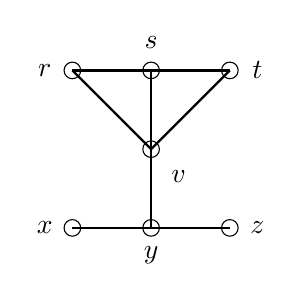
\begin{tikzpicture}
        \draw[fill=white] (0,0) circle (3pt);
        \draw[fill=white] (0,2) circle (3pt);
        \draw[fill=white] (1,0) circle (3pt);
        \draw[fill=white] (1,1) circle (3pt);
        \draw[fill=white] (1,2) circle (3pt);
        \draw[fill=white] (2,0) circle (3pt);
        \draw[fill=white] (2,2) circle (3pt);

        \node at (0-.35,0) {$x$};
        \node at (0-.35,2) {$r$};
        \node at (1,0-.35) {$y$};
        \node at (1+.35,1-.35) {$v$};
        \node at (1,2.35) {$s$};
        \node at (2.35,0) {$z$};
        \node at (2.35,2) {$t$};

        \draw[thick] (0,2) -- (1,2) -- (2,2);
        \draw[thick] (0,0) -- (1,0) -- (1,1) -- (1,2);
        \draw[thick] (1,0) -- (2,0);
        \draw[thick] (2,2) -- (1,1) -- (0,2);
    \end{tikzpicture}

\bigskip
\noindent{\bf 1.12}

\noindent{\bf (a)}

    $(x, u, v, r, u, x, y)$

\noindent{\bf (b)}

    $(v, s, t, v, w)$

\noindent{\bf (c)}

    Impossible. In order for such a path to exist, $r$ would need to have a neighbor that is neighbors with $z$. None of $r$'s neighbors are neighbors with $z$.

\noindent{\bf (d)}

    Impossible. In order for such a path to exist, $x$ would need to have a neighbor in common with either of $z$'s neighbors, $y$ and $w$. $x$'s neighbors have no overlap with the neighbors of $y$ and $w$.
    
\noindent{\bf (e)}

    $(x, y, v, t)$

\noindent{\bf (f)}

    $(r, v, t, w, z, y, x, u, v, s, r)$

\noindent{\bf (g)}

    $(x, y, z, w, t, s, r, u, x)$

\newpage
\noindent{\bf 1.18}

\noindent{\bf (a)}

    $c_3$ and $c_{11}$ are adjacent to $c_1$ in $G$.

\noindent{\bf (b)}

    $c_4$, $c_6$, and $c_{11}$ are adjacent to $c_2$ in $G$.

\noindent{\bf (c)}

    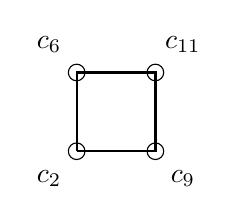
\begin{tikzpicture}
        \draw[fill=white] (0,0) circle(3pt);
        \draw[fill=white] (0,1) circle(3pt);
        \draw[fill=white] (1,0) circle(3pt);
        \draw[fill=white] (1,1) circle(3pt);

        \node at (-.35, -0.35) {$c_2$};
        \node at (-.35, 1.35) {$c_6$};
        \node at (1.35, -0.35) {$c_9$};
        \node at (1.35, 1.35) {$c_{11}$};

        \draw[thick] (0,0) -- (0,1) -- (1,1) -- (1,0) -- (0,0);
    \end{tikzpicture}

\noindent{\bf (d)}

    $(c_1, c_3, c_5, c_8, c_7)$

\bigskip
\begin{proof}
    Let $R$ be an equivalence relation on a nonempty set $A$, and let $a,b \in A$ such that $[a] \cap [b] \neq \emptyset$.
    We claim that $[a] = [b]$.
    Since $[a] \cap [b] \neq \emptyset$, there exists $c \in [a] \cap [b]$.
    Let $x \in [a]$, and let $y \in [b]$.
    Since $c \in [a]$ and $c \in [b]$, $c R a$ and $c R b$.
    Thus, since $x \in [a]$ and $y \in [b]$, $x R a$ and $y R b$.
    Then, since $R$ is symmetric, $a R c$ and $b R y$.
    Therefore, by transitivity, $x R c$.
    By transitivity, $x R b$. % Fix wording here.
    By transitivity, $x R y$.
    Consequently, since $R$ is symmetric, $y R x$.
    Thus, $[a] = [b]$.
\end{proof}

\end{document}